\section{Algunas propiedades de las bases de Legendre discretas}

Fijada una dimensión $n$, estudiaremos algunas propiedades
de la base de Legendre discreta $\cali{L}^{n}$ definida en 
\ref{def: base de Legendre discreta}, que mostraran la utilidad
de considerar representaciones de señales finitas
respecto a la base
$\cali{L}^{n}$ frente a otras bases ortonormales del espacio, pues
a diferencia de una BON cualquiera de $\IR^{n}$, como detallaremos
en la subsección 
\ref{Caracterización de la morfología en términos de coeficientes respecto a la base de Legendre discreta},
$\cali{L}^{n}$ satisface no sólo el primer punto
de la lista de objetivos
\ref{lista de objetivos}, sino también el segundo, el 
correspondiente a la morfología.

En la subsección 
\ref{Relación entre proyecciones a espacios de polinomios discretos y aproximaciones por mínimos cuadrados}
estudiamos la estrecha relación que existe entre
proyecciones a los espacios $W_{n,i}$ y a aproximaciones
polinomiales de mínimos cuadrados.

Terminamos con la subsección \ref{subsec: ejemplos},
en la que se presentan algunos ejemplos en 
dimensiones concretas.

\subsection{Caracterización de la morfología en términos de coeficientes respecto a la base de Legendre discreta}
\label{Caracterización de la morfología en términos de coeficientes respecto a la base de Legendre discreta}
Ahora que contamos con bases ortonormales
para los espacios de polinomios discretos
(c.f. corolario \ref{cor: BON de legendre para espacios Wk}),
es sencillo reescribir al corolario
\ref{cor: condiciones necesarias y suficientes para que x sea afín en términos de pertenencia a espacios Wi},
en el que se dan condiciones necesarias y suficientes para que
una señal sea afín o cuadrática,
no en términos de pertenencia a espacios de polinomios
discretos,
sino en términos de coeficientes.

\begin{obs} \label{obs: condiciones necesarias y suficientes sobre la forma de x en terminos de los espacios Wi}
Sean $n \in \IN$, $\cali{L}^{n}$
la base de Legendre discreta de dimensión $n$
definida en 
\ref{def: base de Legendre discreta}, 
$x \in \IR^{n}$ una señal de dimensión $n$, y
\[
a_{k}=<x, \cali{L}^{n,k}>, \hspace{0.2cm} 0 \leq k \leq n-1
\]
los coeficientes de $x$
respecto
\footnote{Los productos punto entre $x$
y los elementos de la base de Legendre discreta
son, en efecto, los coeficientes de $x$
respecto a $\cali{L}^{n}$ por ser
esta última una BON de $\IR^{n}$.
\TODO{referencia al apéndice.}} a $\cali{L}^{n}$,
de tal forma que se tiene la descomposición
\begin{equation}
\label{eq5: 1Dic}
x=\suma{k=0}{n-1}{a_{k}\cali{L}^{n,k}}.
\end{equation}


Se tiene que la señal $x$ es
 
\begin{itemize}
\item constante si y sólo si para todo índice
$1 \leq k \leq n-1$ se cumple que $a_{k}=0$,

\item afín si y sólo si sólo sus primeros
para todo índice
$2 \leq k \leq n-1$ se cumple que $a_{k}=0$,

\item cuadrática si y sólo si 
para todo índice
$3 \leq k \leq n-1$ se cumple que $a_{k}=0$,
y además $a_{2} \neq 0$.
\end{itemize}
\end{obs}

Más aún; a pesar de que
una señal $x$ no sea ni lineal ni cuadrática, gracias a la 
ortogonalidad de la base
$\cali{L}^{n}$ podemos formalizar lo que
entendemos por que una señal se asemeje a ser
afín o cuadrática y, además, \textbf{cuantificar} esta semejanza;
profundizaremos más adelante estas ideas
en la subsección \ref{subsec: ejemplos},
pero esbozamos ahora a grandes rasgos la idea:
dada una señal $x \in \IR^{n}$, es fácil expresar
a $x$ como combinación lineal
de elementos de $\cali{L}^{n}$ 
(pues esto se reduce a calcular $n$ productos punto),
o sea, llegar a una expresión de la forma
\eqref{eq5: 1Dic}; como se explica en 
la observación 
\ref{obs: condiciones necesarias y suficientes sobre la forma de x en terminos de los espacios Wi}, tenemos condiciones necesarias y suficientes
(muy sencillas de comprobar)
\textbf{en términos de los coeficientes $a_{k}$}
de \eqref{eq5: 1Dic} en referencia a la \textbf{forma
de la gráfica de $x$}, pero, incluso aunque no se satisfagan
estas condiciones,
seguimos pudiendo \TODO{... Parseval. Tal vez esto
debería ir en el apéndice.} 



\noindent A la luz del teorema de la proyección ortogonal, 
las proyecciones de $x$ sobre los espacios 
$W_{n,0}$, $W_{n,1}$
y $W_{n,2}$ son los vectores
de estos espacios más cercanos (en términos de la 
distancia euclidea usual)
a $x$; es natural entonces formular
las siguientes definiciones.


\begin{defi}
Si $x \in \IR^{n}$ y
\begin{equation}
\label{eq0: 5Dic}
\Pi_{W_{n,i}}: \IR ^{n}  \longrightarrow W_{i}, \hspace{0.2cm}
i=0,1,2
\end{equation}
son las proyecciones ortogonales
\sidenote{Puede recordar la definición
de proyección ortogonal, basada en la unicidad
establecida en el 
teorema de la proyección ortogonal \label{Teo:proyOrt},
en \eqref{eq3: 1Dic}.}
a los espacios 
$W_{n,0}$, $W_{n,1}$ y $W_{n,2}$, a los vectores
\[
\Pi_{W_{n,i}}(x), \hspace{0.2cm} i=0,1,2
\]
les llamaremos la \textbf{parte constante}
o \textbf{promedio}, la \textbf{parte afín} y la
\textbf{parte cuadrática}, respectivamente, de $x$.
\end{defi}

\begin{prop}
Sea $x \in \IR^{n}$; si
\[
x= \suma{k=0}{n-1}{a_{k}\cali{L}^{n,k}},
\]
entonces, para toda $0 \leq i \leq n-1$,
\[
\Pi_{W_{n,i}}(x)=\suma{k=0}{i}{a_{k}\cali{L}^{n,k}}.
\]
\end{prop}
\textbf{Demostración.}
Sólo recuerde que, para toda $0 \leq i \leq n-1$,
los vectores $\cali{L}^{n, j}$ con $0 \leq j \leq i$
conforman una BON de $W_{n,i}$
(c.f. corolario \ref{cor: BON de legendre para espacios Wk}) y
que $a_{k}= \langle x, \cali{L}^{n,j} \rangle$.
Use el corolario \ref{cor: proyeccion en terminos de una BON}.
\QEDB 
\vspace{0.2cm}

\subsection{Relación entre proyecciones a espacios de polinomios discretos y aproximaciones por mínimos cuadrados}
\label{Relación entre proyecciones a espacios de polinomios discretos y aproximaciones por mínimos cuadrados}

Hasta el momento, hemos partido siempre
de una señal $x \in \IR^{n}$
y, a partir de ella, considerado al subconjunto $G_{x}$ 
de $\IR^{2}$ (interesándonos por patrones de 
recta y parábola que este pueda seguir).
Si, recíprocamente, se tiene un 
subconjunto de puntos de $\IR^{2}$ 
\begin{equation}
\label{eq: Halloween!}
G:=\{(j, x_{j}): 0 \leq j \leq n-1 \},
\end{equation}
con $n \geq 2$,
cuyas abscisas formen una malla uniforme
de $n$ puntos, tenemos ahora dos caminos
para dar una aproximación lineal
que modele el comportamiento 
seguido por estos puntos:

\begin{enumerate}
\item El clásico método de
mínimos cuadrados, método que, en este contexto,
consiste en minimizar a la función
de dos variables 
\begin{equation}
\label{eq: funcion a minimizar}
\mu (m,b)= \suma{j=1}{n}{(x_{j}-(mj+b))^{2}},
\end{equation}
es decir, en encontrar una pendiente
$m_{0} \in \IR$ y un $b_{0} \in \IR$ 
para los que la suma de las distancias
al cuadrado entre las mediciones 
(i.e. los valores $x_{j}$)
y los valores correspondientes de la función
$l_{min}(x):=m_{0}x+b_{0}$
sea mínima. 


\begin{figure}[H]
	\sidecaption{
	Partimos del conjunto $G$
	cuyos elementos son $(0, 5)$,
	$(1, 3.2)$, $(2, 4.6)$, $(3,0)$
	y $(4,-0.3)$, y
	calculamos la
	recta de mínimos cuadrados correspondiente
	a este conjunto, que resulta ser 
	$l_{min}=-1.38x+5.26$.
	\label{fig: proyeccion vs minimos cuadrados 1}
	}
	\centering
	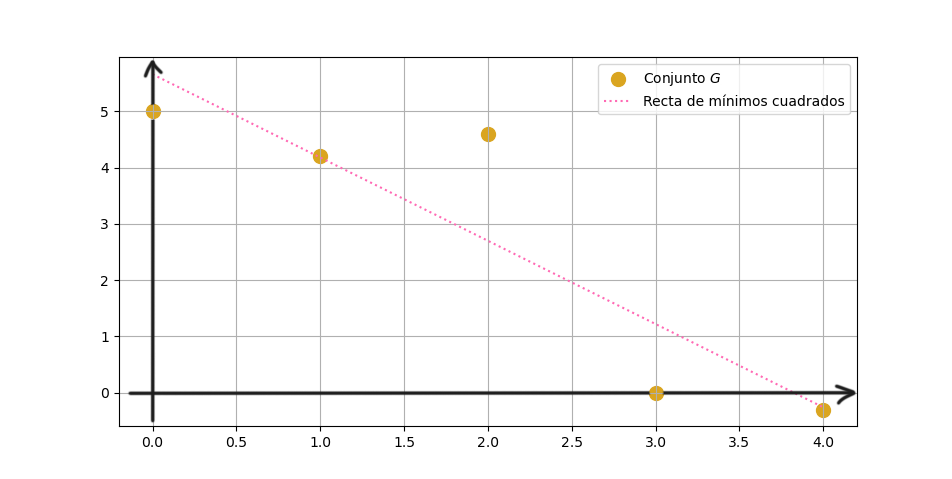
\includegraphics[scale= 0.5]{2Dic_1} 
\end{figure}	


\item Considerar al vector $x=(x_{j})_{j=0}^{n-1}$
de $\IR^{n}$, proyectarlo al espacio $W_{n,1}$ 
de polinomios discretos de dimensión $n$ y grado uno,
\footnote{\TODO{ver si siempre hablo de la dimensión
de un polinomio discreto. Esto es importante.}}
y usar
a la recta $l_{x}$ cuya discretización en 
$\cali{P}_{n}$ sea esta proyección
$\Pi_{W_{n,1}}(x) \in W_{n,1}$ 
(que existe por ser precisamente
$W_{n,1}$ el espacio de discretizaciones
de polinomios discretos de dimensión $n$ con
grado a lo más uno, c.f. 
teorema \ref{cor: propiedades importantes de espacios Wi})
como aproximación lineal del conjunto \eqref{eq: Halloween!}.


\begin{figure}[H]
	\sidecaption{	
		El vector formado a partir
		del conjunto $G$ 
		de la figura 
		\ref{fig: proyeccion vs minimos cuadrados 1}
		es $x=(5,3.2,4.6,0,-0.3)$.
		Su proyección al espacio $W_{5,1}$ es
		$\Pi_{W_{5,1}}(x)= (5.26, 3.88,
		2.5, 1.12, -0.26)$, y la recta
		cuya discretización en $\cali{P}_{5}$	
		es la señal $\Pi_{W_{5,1}}(x)$ es
		$l_{x}=-1.38x+5.26$.
	\label{fig: proyeccion vs minimos cuadrados 2}
	}
	\centering
	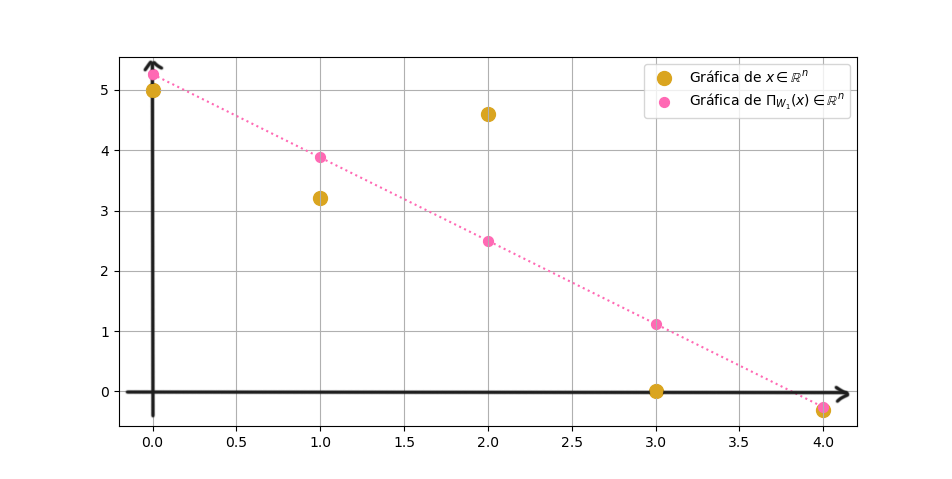
\includegraphics[scale= 0.5]{2Dic_2 } 
\end{figure}	

\end{enumerate}


Puesto que el mínimo 
$(m_{0}, b_{0})$ de la función 
\eqref{eq: funcion a minimizar} siempre existe,
y como siempre puede formarse el vector
$x=(x_{j})_{j=0}^{n-1}$ a partir del conjunto $G$
dado en \eqref{eq: Halloween!} 
y proyectarse este
a $W_{n,1}$, los dos caminos discutidos arriba
son siempre realizables.


\noindent Como establecemos en la siguiente observación, estas
dos formas de abordar el problema de aproximación
coinciden. Observe que la demostración de este hecho 
no es más que una consecuencia directa del 
teorema de la proyección \ref{Teo:proyOrt}
pues, hablando en los términos que hemos
usado hasta ahora, encontrar la recta de mínimos
cuadrados de la 
gráfica $G_{x}$ es lo mismo que encontrar al elemento
del espacio $W_{n,1}$ cuya distancia euclidea a $x \in \IR^{n}$
sea mínima.


\begin{prop}
Sea $n \geq 2$ y sea el conjunto de $n$ puntos del plano
\begin{equation}
\label{eq10: 10Dic}
\{(j, x_{j}): 0 \leq j \leq n-1 \}
\subseteq \IR^{2}.
\end{equation}
Si $x=(x_{j})_{j=0}^{n-1}$ es la señal cuya
gráfica $G_{x}$ coincide con el conjunto dado
en \eqref{eq10: 10Dic}, si
\begin{itemize}
\item $l_{min}= m_{0}x+b_{0}$ es la recta obtenida 
aproximando los puntos del conjunto 
\eqref{eq10: 10Dic}
con el método de mínimos cuadrados, y

\item $l_{x}$ es la recta cuya versión discreta 
respecto a la malla uniforme $\cali{P}_{n}$
es $\Pi_{W_{n,1}}(x) \in \IR^{n}$, 

\end{itemize} 
entonces las rectas $l_{x}$ y $l_{min}$ coinciden.
\end{prop}
\noindent 
\textbf{Demostración.}
Si demostramos que las señales
\[
r:= \Omega_{n, \cali{P}_{n}}(l_{min}) \in \IR^{n}
\]
y
\[
\Pi_{W_{n,1}}(x) \in W_{n,1} \subseteq \IR^{n}
\]
coinciden, podremos concluir la 
igualdad entre las rectas $l_{x}$ y $l_{min}$
(pues la igualdad $r= \Pi_{W_{n,1}}(x)$
significa que las rectas $l_{min}$ y $l_{x}$
{coinciden en los puntos con abscisas los elementos
de $\cali{P}_{n}$, que son al menos dos).

Por ser $r$ la discretización
en una malla uniforme de un
polinomio de grado uno, es elemento del espacio $W_{n,1}$
(c.f. teorema 
\ref{cor: propiedades importantes de espacios Wi}). 
Además, si $z$ es cualquier señal afín
(es decir, cualquier elemento de $W_{n,1}$)
y si $y=mx+b$
es la ecuación de la recta sobre la que yace su gráfica,
por definición de $l_{min}$ sabemos que

\begin{equation}
\label{eq0: 5Enero}
\suma{j=1}{n}{(x_{j}-(m_{0}j+b_{0}))^{2}}
=\mu(m_{0}, b_{0}) \leq \mu(m, b)= 
\suma{j=1}{n}{(x_{j}-(mj+b))^{2}};
\end{equation}
\noindent 
tomando raíces cuadradas 
en ambos extremos de \eqref{eq0: 5Enero}
llegamos a la desigualdad
\[
d(x, r) \leq d (x,z)
\]
(donde $d$ denota a la distancia euclidea en $\IR^{n}$).
Como $z$ fue un elemento arbitrario del espacio $W_{n,1}$,
inferimos que

\[
d(x, r)  = \text{inf} \{ d (x,z) : z \in W_{n,1} \};
\]
de la unicidad establecida en el teorema de la proyección
ortogonal \ref{Teo:proyOrt} concluimos que $r= \Pi_{W_{n,1}}(x)$. \QEDB
\vspace{0.2cm}


En esta subsección
tratamos sólo caso lineal, pero,
naturalmente, discusiones
totalmente análogas se valen para grados más altos
(estando los grados posibles acotados superiormente
por la cardinalidad del conjunto de puntos $G$
dado en \eqref{eq: Halloween!} 
a aproximar), por 
ejemplo, cuando se buscan
aproximaciones cuadráticas
(resp. cúbicas) para cuando
la cardinalidad del conjunto 
\eqref{eq: Halloween!} es mayor o igual a tres 
(resp. cuatro).